\documentclass[12pt]{article}
\usepackage[paper=letterpaper,margin=1.5cm]{geometry}
\usepackage{amsmath}
\usepackage{amssymb}
\usepackage{amsfonts}
\usepackage{mathtools}
%\usepackage[utf8]{inputenc}
%\usepackage{newtxtext, newtxmath}
\usepackage{lmodern}     % set math font to Latin modern math
\usepackage[T1]{fontenc}
\renewcommand\rmdefault{ptm}
%\usepackage{enumitem}
\usepackage[shortlabels]{enumitem}
\usepackage{titling}
\usepackage{graphicx}
\usepackage[colorlinks=true]{hyperref}
\usepackage{setspace}
\usepackage{subfigure} 
\usepackage{braket}
\usepackage{color}
\usepackage{tabularx}
\usepackage[table]{xcolor}
\usepackage{listings}
\usepackage{mathrsfs}
\usepackage{stackengine}
\usepackage{physics}
\usepackage{afterpage}
\usepackage{pdfpages}
\usepackage[export]{adjustbox}
\usepackage{biblatex}

\setstackEOL{\\}

\definecolor{dkgreen}{rgb}{0,0.6,0}
\definecolor{gray}{rgb}{0.5,0.5,0.5}
\definecolor{mauve}{rgb}{0.58,0,0.82}


\lstset{frame=tb,
  language=Python,
  aboveskip=3mm,
  belowskip=3mm,
  showstringspaces=false,
  columns=flexible,
  basicstyle={\small\ttfamily},
  numbers=none,
  numberstyle=\tiny\color{gray},
  keywordstyle=\color{blue},
  commentstyle=\color{dkgreen},
  stringstyle=\color{mauve},
  breaklines=true,
  breakatwhitespace=true,
  tabsize=3
}
\setlength{\droptitle}{-6em}

\makeatletter
% we use \prefix@<level> only if it is defined
\renewcommand{\@seccntformat}[1]{%
  \ifcsname prefix@#1\endcsname
    \csname prefix@#1\endcsname
  \else
    \csname the#1\endcsname\quad
  \fi}
% define \prefix@section
\newcommand\prefix@section{}
\newcommand{\prefix@subsection}{}
\newcommand{\prefix@subsubsection}{}
\renewcommand{\thesubsection}{\arabic{subsection}}
\makeatother
\DeclareMathOperator*{\argmin}{argmin}
\newcommand{\partbreak}{\begin{center}\rule{17.5cm}{2pt}\end{center}}
\newcommand{\alignbreak}{\begin{center}\rule{15cm}{1pt}\end{center}}
\newcommand{\tightalignbreak}{\vspace{-5mm}\alignbreak\vspace{-5mm}}
\newcommand{\hop}{\vspace{1mm}}
\newcommand{\jump}{\vspace{5mm}}
\newcommand{\R}{\mathbb{R}}
\newcommand{\C}{\mathbb{C}}
\newcommand{\N}{\mathbb{N}}
\newcommand{\G}{\mathbb{G}}
\renewcommand{\S}{\mathbb{S}}
\newcommand{\bt}{\textbf}
\newcommand{\xdot}{\dot{x}}
\renewcommand{\star}{^{*}}
\newcommand{\ydot}{\dot{y}}
\newcommand{\lm}{\mathrm{\lambda}}
\renewcommand{\th}{\theta}
\newcommand{\id}{\mathbb{I}}
\newcommand{\si}{\Sigma}
\newcommand{\Si}{\si}
\newcommand{\inv}{^{-1}}
\newcommand{\T}{^\intercal}
\renewcommand{\tr}{\text{tr}}
\newcommand{\ep}{\varepsilon}
\newcommand{\ph}{\varphi}
%\renewcomand{\norm}[1]{\left\lVert#1\right\rVert}
\definecolor{cit}{rgb}{0.05,0.2,0.45}
\addtolength{\jot}{1em}
\newcommand{\solution}[1]{

\noindent{\color{cit}\textbf{Solution:} #1}}

\newcounter{tmpctr}
\newcommand\fancyRoman[1]{%
  \setcounter{tmpctr}{#1}%
  \setbox0=\hbox{\kern0.3pt\textsf{\Roman{tmpctr}}}%
  \setstackgap{S}{-.9pt}%
  \Shortstack{\rule{\dimexpr\wd0+.1ex}{.9pt}\\\copy0\\
              \rule{\dimexpr\wd0+.1ex}{.9pt}}%
}

\newcommand{\Id}{\fancyRoman{2}}

% Enter the specific assignment number and topic of that assignment below, and replace "Your Name" with your actual name.
\title{STAT 30900: Homework 2}
\author{Caleb Derrickson}
\date{October 31, 2023}

\begin{document}
\onehalfspacing
\maketitle

{\color{cit}\vspace{2mm}\noindent\textbf{Collaborators:}} The TA's of the class, as well as Kevin Hefner, and Alexander Cram.

\tableofcontents

\newpage
\section{Problem 1}
The files required for this problem can be found in the subfolder hw2 in Canvas. The matrix in processed.mat (Matlab format) or processed.txt (comma separated, plain text) is a 49 × 7 matrix where each row is indexed by a country in row.txt and each column is indexed by a demographic variable in column.txt, ordered as in the respective files. So for example, if we denote the matrix by

\[
A 
= 
\begin{bmatrix}\textbf{a}_1^T \\ \textbf{a}_2^T \\ \vdots \\ \textbf{a}_{49}^T\end{bmatrix}
=
\begin{bmatrix} \textbf{$\alpha$}_1,&\dots,&\textbf{$\alpha$}_7\end{bmatrix}
=
\begin{bmatrix}
    a_{11} &a_{12} &\dots &a_{17} \\
    a_{21} &a_{22} &\dots &a_{27} \\
    \vdots &\vdots &\ddots &\vdots \\
    a_{49,1} &a_{49,2} &\dots &a_{49,7}
\end{bmatrix}
\in \R^{49\times 7},
\]
then $a_{23}$ = -0.2743 is Austria’s population per square kilometers (row index 2 = Austria, column index 3 = population per square kilometers). As you probably notice, this matrix has been slightly preprocessed. If you want to see the raw data, you can find them in raw.txt (e.g. the actual value for Austria’s population per square kilometers is 84) but you don’t need the raw data for this problem.

\subsection{Problem 1, part a}
Show that to plot the projections of the row vectors (i.e., samples) $\textbf{a}_1, ..., \textbf{a}_{49} \in \R^{7}$ onto the two-dimensional subspace span $\{ \textbf{v}_j, \textbf{v}_k \cong \R^2\}$, we may simply plot the $n$ points 
\[
    \{(\sigma_ju_{ij}, \sigma_ku_{ik}) \in \R^2 : i = 1, ..., 49\}
\]
where $U = [u_{ij}] \in \R^{49\times 49}$ and $\Sigma = $ diag$(\sigma_1, ..., \sigma_p) \in \R^{49 \times 7}$ are the matrix of left singular vectors and matrix of singular values respectively.  

\partbreak
\begin{solution}

     Denote the Singular Value Decomposition of $A$ as $U\si V^t$, where $U, V$ are matrices constructed by orthonormal vectors. They are related to each other by $A\textbf{v}_k = \sigma_k\textbf{u}_k$, where $\textbf{u}_k, \textbf{v}_k$ is the $k-$th column vector of $U$ and $V$, respectively, and $\sigma_k$ is the $k$-th singular value of $A$. Similarly, $A^*\textbf{u} = \sigma_k\textbf{v}_k$. Thus, if there were some other $\textbf{u}_i$, such that $A^*\textbf{u}_i = \sigma_i\textbf{v}_k$, then 
     \[
     \textbf{v}_k^*\textbf{v}_k = (\frac{1}{\sigma_i}A^*\textbf{u}_i)^*A^*\textbf{u}_k = \frac{1}{\sigma_i}\textbf{u}_i^*AA^*\textbf{u}_k = \frac{\sigma_k^2}{\sigma_i}\textbf{u}_i^*\textbf{u}_k = 0
     \]

      since the set of \textbf{u} vectors are orthonormal Thus, no other $\textbf{u}$ contributes to $\textbf{v}_k$, meaning if we want to project onto the given subspace, we only need to plot $\{(\sigma_ju_{ij}, \sigma_ku_{ik}) \in \R^2 : i = 1, ..., 49\}$.
\end{solution}

\newpage
\subsection{Problem 1, part b}
Find the first two right singular vectors of $A, \textbf{v}_1, \textbf{v}_2 \in \R^7$ . Project the data onto the two-dimensional space span$\{\textbf{v}_1, \textbf{v}_2\} \cong \R^2$ . Plot this in a graph where the x- and y-axes correspond to $\textbf{v}_1$ and $\textbf{v}_2$ respectively and where the points correspond to the countries — label each point by the country it corresponds to. Identify the two obvious outliers.
\partbreak
\begin{solution}

    I will provide the plot below, followed by the code. It seems the two countries I found as outliers are Singapore and Hong Kong.

    \begin{figure}[h]
        \centering
        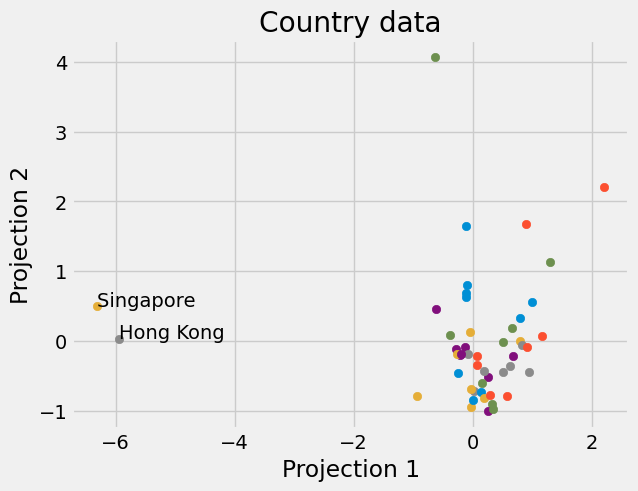
\includegraphics[width = 0.5\textwidth]{Images/problem 1b plot.png}
        \label{fig:problem 1b}
    \end{figure}

\begin{lstlisting}    
import pandas as pd
import numpy as np
import matplotlib.pyplot as plt

#filepaths for country data, names
filepathmat = 'datafiles/processed.txt'
filepathcont = 'datafiles/row.txt'
filepathdemvar = 'datafiles/column.txt'

#read in country names, then data with index as names
cont = pd.read_csv(filepathcont, header=None)
demvar = pd.read_csv(filepathdemvar, header=None)
df = pd.read_csv(filepathmat, header=None)
df = df.set_axis(cont[0], axis='index')

#Write to numpy array to do SVD
df_arr = df.to_numpy()
U, S, V = np.linalg.svd(df_arr)

testpts = []

j, k = 1, 2
for pts in range(U.shape[0]):
    testpts.append((S[j] *U[pts][j], S[k]*U[pts][k]))
pts = np.array(testpts)

#Finding outliers
outlier1 = np.argmin(pts[:, 0])
outpt1 = (outlier1, pts[outlier1, :])
outlier2 = np.argmin(np.delete(pts[:, 0], outlier1))
outpt2 = (outlier2, pts[outlier2, :])

outliers = np.array([df.index[outlier1], df.index[outlier2]])

for x, y in pts:
    plt.scatter(x, y)
    
plt.title("Country data")
plt.style.use('fivethirtyeight')
plt.gray
plt.ylabel(f'Projection {j}')
plt.xlabel(f'Projection {k}')
#Labelling outliers on plot
plt.annotate(f'{outliers[0]}', xy=(outpt1[1]) )
plt.annotate(f'{outliers[1]}', xy=(outpt2[1]) )
\end{lstlisting}
\end{solution}


\newpage
\subsection{Problem 1, part c}
Now do the same with the two left singular vectors of $A$, $\textbf{u}_1, \textbf{u}_2 \in \R^{49}$. Project the column vectors (i.e., variables) $\alpha_1, ..., \alpha_7 \in \R^{49}$ onto the two-dimensional space span$\{\textbf{u}_1, \textbf{u}_2\} \cong \R^2$ and plot this in a graph as before. Note that in this case, the points correspond to the demographic variables — label them accordingly.
\partbreak
\begin{solution}

The plot will be provided below, as well as the code. 

\begin{figure}[h]
    \centering
    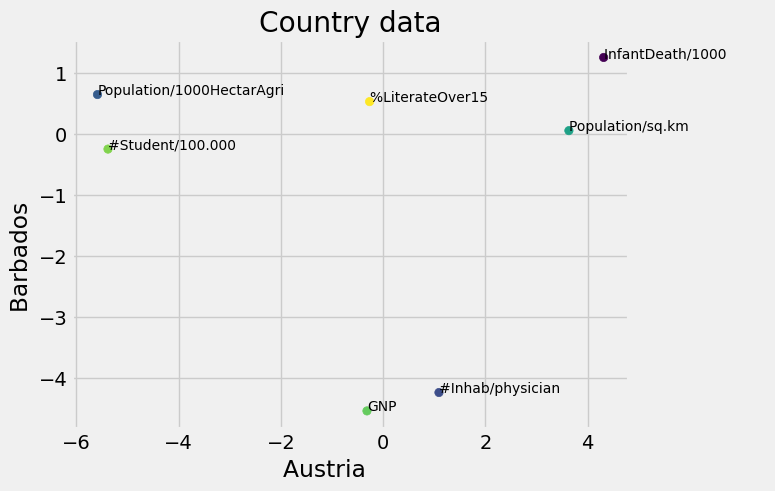
\includegraphics[width = 0.5\textwidth]{Images/problem 1c plot.png}
    \label{fig:problem1c}
\end{figure}

\begin{lstlisting}
#Doing the same except for demographic variables
testpts = []

j, k = 1, 2
for pts in range(V.shape[0]):
    testpts.append((S[j] *V[pts][j], S[k]*V[pts][k]))
pts = np.array(testpts)


# Create the scatter plot
plt.scatter(pts[:, 0], pts[:, 1], c = [random.randint(0, x*10) for x in range(len(V))])

#Finding outliers
for i, (x, y) in enumerate(pts):
    plt.annotate(f'{demvar[0][i]}', xy=(x, y), fontsize=10)

plt.title("Country data")
plt.style.use('fivethirtyeight')
plt.gray
plt.ylabel(f'{df.index[k]}')
plt.xlabel(f'{df.index[j]}')
\end{lstlisting}
\end{solution}

\newpage
\section{Problem 2}
Let $A, B \in \R^{m \times n}$ where $A$ has full column rank.

\subsection{Problem 2, part a}
Show that 
\[
\min_{X \in \R^{n\times m}} \norm{AX - \id_m}_F
\]
has a unique solution. What is the minimum length solution, i.e., where $\norm{X}_F$ is minimum?

\newpage
\section{Problem 3}
Let $A \in \C^{m\times n}$ and $\textbf{b} \in \C^m$. We will discuss a variant of $A\textbf{x} \approx \textbf{b}$ where the error occurs only in $A$. Note that in ordinary least squares we assume that the error occurs only in \textbf{b} while in total least squares we assume that it occurs in both $A$ and \textbf{b}.

\subsection{Problem 3, part a}
Show that if $0 \neq \textbf{x} \in \C^n$, then
\[
\norm{A\Big( \id - \frac{\textbf{x}\textbf{x}^*}{\textbf{x}^*\textbf{x}}\Big)}_F^2 = \norm{A}_F^2 - \frac{\norm{A\textbf{x}}_2^2}{\textbf{x}^*\textbf{x}}
\]
\partbreak
\begin{solution}

 Taking the left side, the following steps can be shown:

\vspace{-5mm}
 \alignbreak
 {\small
 \begin{align}
     \norm{A\Big( \id - \frac{\textbf{x}\textbf{x}^*}{\textbf{x}^*\textbf{x}}\Big)}_F^2 &= \tr \Big[ \Big( A - A\frac{\textbf{x}\textbf{x}^*}{\textbf{x}^*\textbf{x}}\Big)^*\Big( A - A \frac{\textbf{x}\textbf{x}^*}{\textbf{x}^*\textbf{x}}\Big) \Big] &\text{(Trace of Frobenius norm.)}\nonumber\\
     &= \tr \Big[ A^*A\Big] - \tr \Big[ A^*A\frac{\textbf{x}\textbf{x}^*}{\textbf{x}^*\textbf{x}} \Big] - \tr \Big[ \Big( A\frac{\textbf{x}\textbf{x}^*}{\textbf{x}^*\textbf{x}}\Big)^*A\Big] + \tr \Big[ \Big(A\frac{\textbf{x}\textbf{x}^*}{\textbf{x}^*\textbf{x}} \Big)^*A\frac{\textbf{x}\textbf{x}^*}{\textbf{x}^*\textbf{x}}\Big] &\text{(Expanding.)}\nonumber\\
     &= \norm{A}_F^2 - \frac{\norm{\textbf{x}}_2^2}{\norm{\textbf{x}}_2^2}\tr \Big[ A^*A\Big] - \frac{\norm{\textbf{x}}^2_2}{\norm{\textbf{x}}_2^2} \tr \Big[ A^*A\Big] +  \tr \Big[ \frac{\textbf{x}\textbf{x}^*A^*A\textbf{x}\textbf{x}^*}{\textbf{x}^*\textbf{x}\textbf{x}^*\textbf{x}}\Big]&\text{(Simplifying.)}\nonumber\\
     &= \norm{A}_F^2 - 2\norm{A}_2^2 + \frac{\norm{\textbf{x}}_2^2\norm{A}_2^2\norm{\textbf{x}}^2_2}{\norm{\textbf{x}}_2^2 \norm{\textbf{x}}_2^2} &\text{(2-norm definition.)}\nonumber\\
     &= \norm{A}_F^2 - A^*A &\text{(2-norm definition.)}\nonumber\\
     &= \norm{A}_F^2 - \frac{\textbf{x}^*A^*A\textbf{x}}{\textbf{x}^*\textbf{x}} &\text{(2-norm definition.)} \nonumber\\
     &= \norm{A}_F^2 - \frac{\norm{A\textbf{x}}_2^2}{\textbf{x}^*\textbf{x}} &\text{(Simplifying.)}\nonumber
 \end{align}
 }%
 \alignbreak

 There might have been a simpler way to show this, and less questionable, but I believe these steps are valid. 
\end{solution}

\newpage
\subsection{Problem 3, part b}
Show that the matrix 
\[
E = \frac{(\textbf{b} - A\textbf{x})\textbf{x}^*}{\textbf{x}^*\textbf{x}} \in \C^{m\times n}
\]
has the smallest 2-norm among all $E \in \C^{m\times n}$ that satisfy 
\[
(A + E) \textbf{x} = \textbf{b}
\]
\partbreak
\begin{solution}

 Note that all $E$'s satisfy $E\textbf{x} = \textbf{b} - A\textbf{x}$. To distinguish the $E$ matrices, we'll denote $E'$ as a matrix that satisfies $(A+E')\textbf{x} = \textbf{b}$. Thus, the following can be shown:

 \alignbreak
 \begin{align}
     \norm{E}_2^2 &= \norm{\frac{(\textbf{b} - A\textbf{x})\textbf{x}^*}{\textbf{x}^*\textbf{x}}}^2_2 &\text{(Given.)}\nonumber\\
     &= \Big| \frac{1}{\textbf{x}^*\textbf{x}}\Big|^2 \norm{(\textbf{b} - A\textbf{x})\textbf{x}^*}_2^2 &\text{(Denominator is real.)}\nonumber\\
     &\leq \Big| \frac{1}{\textbf{x}^*\textbf{x}}\Big|^2 \norm{\textbf{b} - A\textbf{x}}_2^2\norm{\textbf{x}^*}_2^2 &\text{(Cauchy Schwartz.)}\nonumber\\
     &= \frac{\norm{\textbf{b} - A\textbf{x}}_2^2}{\norm{\textbf{x}}^2_2} &\text{(Simplifying.)}\nonumber\\
     &= \frac{\norm{E'\textbf{x}}_2^2}{\norm{\textbf{x}}_2^2} &\text{(Equality above.)}\nonumber\\
     &\leq \norm{E'}_2^2 \frac{\norm{\textbf{x}}_2^2}{\norm{\textbf{x}}_2^2} &\text{(Consistency of 2-norm.)}\nonumber\\
     \implies \norm{E}_2^2&\leq \norm{E'}_2^2 &\text{(Simplifying.)}\nonumber\\
     \iff \norm{E}_2 &\leq \norm{E'}_2 \nonumber
 \end{align}
 \alignbreak
\end{solution}

\newpage
\subsection{Problem 3, part c}
Let $A, \textbf{b}, \textbf{x}$ be given and fixed. What are the solutions of 
\[
    \min_{(A+E)\textbf{x} = \textbf{b}} \norm{E}_2 \hspace{3mm} \text{and} \hspace{3mm} \min_{(A+E)\textbf{x} = \textbf{b}} \norm{E}_F
\]
where the minimum is taken over all $E \in \C^{m\times n}$ such that $(A+E)\textbf{x} = \textbf{b}$?
\partbreak
\begin{solution}

We just showed in the previous part that when 
\[
    E = \frac{(\textbf{b} - A\textbf{x})\textbf{x}^*}{\textbf{x}^*\textbf{x}} \in \C^{m\times n}
\] 

 Then $E$ is the smallest of all $E$'s satisfying $A+E)\textbf{x} = \textbf{b}$. We just have to show that this be attained for some $E$. Note by my observation in part b, any $E$ satisfies $E\textbf{x} = \textbf{b} - A\textbf{x}$. Multiplying on the right by $\textbf{x}^*$ yields $E\textbf{x}\textbf{x}^* = (\textbf{b} - A\textbf{x})\textbf{x}^*$. To recover the given equality, we require $E\textbf{x} = \textbf{x}E$, which only happens when $E$ is a multiple of the identity matrix. 
\end{solution}

\newpage
\section{Problem 4}
In the following, $\kappa(A) := \norm{A}\norm{A^\dag}$ for $A\in \C^{m\times n}$ where $\norm{\cdot}$ denotes a submultiplicative matrix norm. We will write $\kappa_p(A)$ if the norm involved is a matrix p-norm. 

\subsection{Problem 4, part a}
Show that for any nonzero $A \in \C^{m\times n}$, $\kappa(A) \geq 1$.

\partbreak
\begin{solution}

 We are given that $\norm{\cdot}$ is submultiplicative, thus $\norm{A}\norm{A^\dag} \geq \norm{AA^\dag}.$ If A is invertible, then $AA^\dag = AA^{-1} = \id$. Note that $\norm{\id} = \norm{\id^2} \leq \norm{\id}^2$, thus $\norm{\id} \geq 1$ for any submultiplicative norm. Then $\kappa(A) = \norm{A}\norm{A^\dag} \geq 1$. If $A$ is not invertible, then we can use SVD. We will write $A = U\Sigma V^*$, so $A^\dag = V\Sigma^\dag U^*$. Then,

 \alignbreak
 \begin{align}
     \norm{AA^\dag} &= \norm{U\Si V^* V \Si ^\dag U^*} &\text{(By SVD.)}\nonumber\\
     &= \norm{U\Si\Si ^\dag U^*} &\text{($V$ is hermitian.)}\nonumber\\
     &= \norm{U\begin{bmatrix}\id_r\\0\end{bmatrix}U^*}, \norm{U\begin{bmatrix}\id_r &0\end{bmatrix}U*} &\text{(Depends if $m \geq n$, or reverse.)}\nonumber\\
     &= \norm{U_rU^*} &\text{(In either case, we take the first r vectors of $U$.)}\nonumber\\
     &= \norm{\id_r} &\text{(Simplifying.)}\nonumber\\
     &\geq 1 &\text{(Identity is $\geq 1$.)}\nonumber
 \end{align}
 \alignbreak

 Note in these steps, I took the first $r$ rows \textit{or} columns from $U$ or $U^*$. Without loss of generality, since $U$ is hermitian, the above is given. Note that $\id_r$ in the last step is an $m \times n$ matrix, which I take its norm as in the $r\times r$ case. 
\end{solution}

\newpage
\subsection{Problem 4, part b}
Show that for any $A \in \C^{m\times n}$,
\[
    \kappa_2(A^*A) = \kappa_2(A)^2
\]
but that in general,
\[
    \kappa(A^*A)\neq \kappa(A)^2
\]
\partbreak
\begin{solution}

 The first statement is just an exercise in algebra, Note I will be using SVD. 

 \alignbreak
 \begin{align*}
     \kappa_2(A^*A) &= \norm{V\Si U^* U\Si V^*}_2 \norm{(V\si U^* U\Si V^*)^\dag} &\text{(SVD of $A$ and $A^*$.)}\nonumber\\
     &= \norm{V\Si^2V^*}_2 \norm{(V\Si ^2V^*)^\dag}_2 &\text{($U$ is orthogonal.)}\nonumber\\
     &= \norm{V\si^2 V^*}_2 \norm{V\si^{2\dag}V^*}_2 &\text{(Pseudo-Inverse of second term.)}\nonumber\\
     &= \norm{\si^2}_2 \norm{\si^{2\dag}}_2 &\text{(2-norm is unitarily invariant.)}\nonumber\\
     &= (\si^2)^*\si^2 (\si^{2\dag})^*\si^{2\dag} &\text{(Writing out 2-norm.)}\nonumber\\
     &= (\si^*\si)^2 ((\si^\dag)^* \si^\dag)^2 &\text{($\si^* = \si$ and $\si^{2\dag} = \si^{\dag 2}$.)}\nonumber\\
     &= \norm{\si}_2^2\norm{\si^\dag}_2^2 &\text{(2-norm definition.)}\nonumber\\
     &= \norm{U\si V^*}^2_2\norm{V\si^\dag U^*}_2^2 &\text{(2-norm is untiarily invariant.)}\nonumber\\
     &= \norm{A}_2^2\norm{A^\dag}_2^2 &\text{(SVD of $A$ and $A^\dag$.)}\nonumber\\
     &= \kappa_2(A)^2 &\text{(Definition of $\kappa_2(A)$).}\nonumber
 \end{align*}
 \alignbreak

 In the above calculations, I used the fact that the 2-norm is unitarily invariant, as well as the property that $\norm{A}_2 = A^*A.$ These properties will not hold true for any general matrix norm.  
\end{solution}

\newpage
\subsection{Problem 4, part c}
Show that for nonsingular $A, B \in \C^{n\times n}$, 
\[
\kappa(AB)\leq \kappa(A)\kappa(B).
\]
 It this true in general without the nonsingular condition?
 \partbreak
 \begin{solution}

     For nonsingular $A, B$, this property is easy to show. Note the pseudoinverse turns into a normal inverse for the product.

     \alignbreak
     \begin{align}
         \kappa(AB) &= \norm{AB}\norm{(AB)^{-1}} &\text{(Given.)}\nonumber\\
         &= \norm{AB} \norm{B^{-1}A^{-1}} &\text{(Inverse of $AB$.)}\nonumber\\
         &\leq \norm{A} \norm{B} \norm{B^{-1}} \norm{A^{-1}} &\text{(Submultiplication.)}\nonumber\\
         \implies \kappa(AB) &\leq \kappa(A)\kappa(B)\nonumber
     \end{align}
     \alignbreak
 \end{solution}

\newpage
 \subsection{Problem 4, part d}
 Let $Q \in \C^{n\times n}$ be a matrix with orthonormal columns. Show that 
 \[
 \kappa_2(Q) = 1.
 \]
 Is this true if $Q$ has orthonormal rows instead? Is this true with $\kappa_1$ or $\kappa_\infty$ in place of $\kappa_2$?
 \partbreak
 \begin{solution}
     
 \end{solution}
\end{document}
